\documentclass[10pt,twocolumn]{article}
\usepackage[margin=0.72in]{geometry}
\usepackage{amsmath,amssymb,booktabs,graphicx,hyperref}
\title{\textbf{State Preparation Is Not Quantum Memory: Exact 256-Branch Verification, 16/16 Post-Preparation Fault Taxonomy, Strict RFC 8785 Provenance, and Hash-Locked Quantinuum H2 Dispatch for $[[16, 2, 4]]$ Wen-Plaquette Codes}}
\author{Devin Phillip Davis\\Agile Defense Systems LLC\\\texttt{OSIRIS-QEC-002 (osiris-qec v1.1.1)} \quad \texttt{DOI: 10.5281/zenodo.24424726} \quad \texttt{https://github.com/quantum-osiris/osiris-qec}}
\date{November 21, 2026 --- Version 1.1.1 (\textbf{STATUS: HARDWARE-UNVALIDATED})}

\begin{document}
\maketitle

\begin{abstract}
\noindent\textbf{Status: HARDWARE-UNVALIDATED.} Fault-tolerant state preparation in a topological stabilizer codespace is operationally distinct from a quantum error-correcting (QEC) memory. Studying the $20$-qubit $[[16,2,4]]$ periodic Wen-plaquette two-round measurement and $7$-entry lookup-table (LUT) feed-forward preparation circuit ($16$ data qubits plus $4$ recycled ancillas; prior art Iqbal \emph{et al.}, arXiv:2302.01917), we show that while weight-$1$ Pauli-$Z$ faults injected \emph{before} preparation are corrected $16/16$ times ($F_L=1.0$), complete $16/16$ \emph{post}-preparation Pauli-$Y$ and Pauli-$Z$ sweeps across all data qubits $q[0..15]$ excite nonzero $X$-syndromes ($16/16$ detected) yet preserve the encoded logical state in $\mathbf{0/16}$ cases ($F_L=0.0$ for $Y$; $<10^{-3}$ for $Z$), and $X$ faults escape detection entirely because $Z$ stabilizers are never measured. Around this scope boundary (benchmark \texttt{OSIRIS-QEC-002}, package \texttt{osiris-qec v1.1.1}), compilation and execution enforce a preregistered artifact lock verifying pre-compile SHA-256 (\texttt{b86aeabd70eecb7f5f...}) and Quantinuum H2-1 ISA SHA-256 (\texttt{02d5cb72849f9b473c...}) both pre-flight and post-compile under \texttt{optimisation\_level=0}. We contribute hardened register-collision and metadata-normalized \texttt{pytket} passes, exact $256$-branch enumeration, dual-basis Qiskit Aer cross-checks, a write-ahead ledger pinned exclusively to IETF RFC~8785 (\texttt{rfc8785==0.1.4}), and \texttt{qnexus} 0.51.4 transport with \texttt{Retry-After} and jittered backoff governed by a per-basis $95\%$ Wilson lower bound $>0.99$.
\end{abstract}

\section{Hardware Allocation and Hardened Pass Contract}
Sixteen vertex data qubits $q[0..15]$ implement the $[[16,2,4]]$ toroidal Wen-plaquette encoding, while $4$ ancilla qubits $q[16..19]$ are recycled via mid-circuit \texttt{Reset} ($24$ \texttt{Measure}, $8$ \texttt{Reset} total; ancillas do not contribute to logical code distance; Fig.~\ref{fig:torus}). \texttt{WenPlaquetteFeedForwardPass} and \texttt{build\_wen\_plaquette} reject non-empty inputs and colliding \texttt{q/qr/quantum/c/creg/cl/classical} registers while normalizing mutable metadata so v1.0.0 (\texttt{10.5281/zenodo.24406733}), v1.1.0 (\texttt{10.5281/zenodo.24421051}), and v1.1.1 circuit hashes match bit-for-bit.

\begin{figure}[t]
\centering
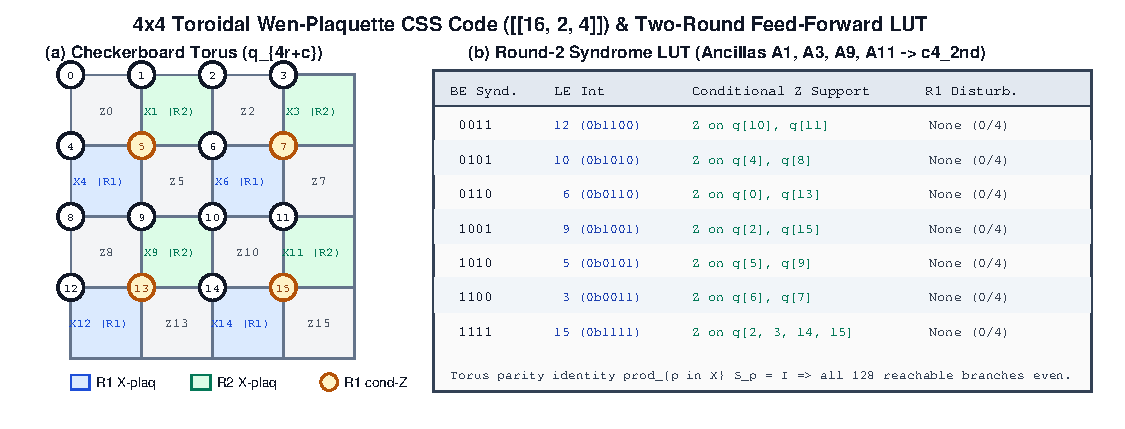
\includegraphics[width=\columnwidth]{fig1_torus_checkerboard_lut.pdf}
\caption{$[[16,2,4]]$ toroidal layout ($16$ data + $4$ recycled ancillas) and $7$-entry Round-2 LUT.}
\label{fig:torus}
\end{figure}

\section{Exact 256-Branch Verification and Noise Benchmark}
Exhaustive $256$-branch enumeration confirms $128/128$ reachable even-parity branches land in $+1$ codespace (worst $\langle S\rangle = 0.9999999999999942$, overlap $0.9999999999999885$ to $|00\rangle_L$), cross-checked in $X$ ($512/512$) and $Z$ ($256/256$) bases on Qiskit Aer and via \texttt{osiris qec run --target selene}. Table~\ref{tab:bench} and Fig.~\ref{fig:bench} report noisy trajectories.

\begin{figure}[t]
\centering
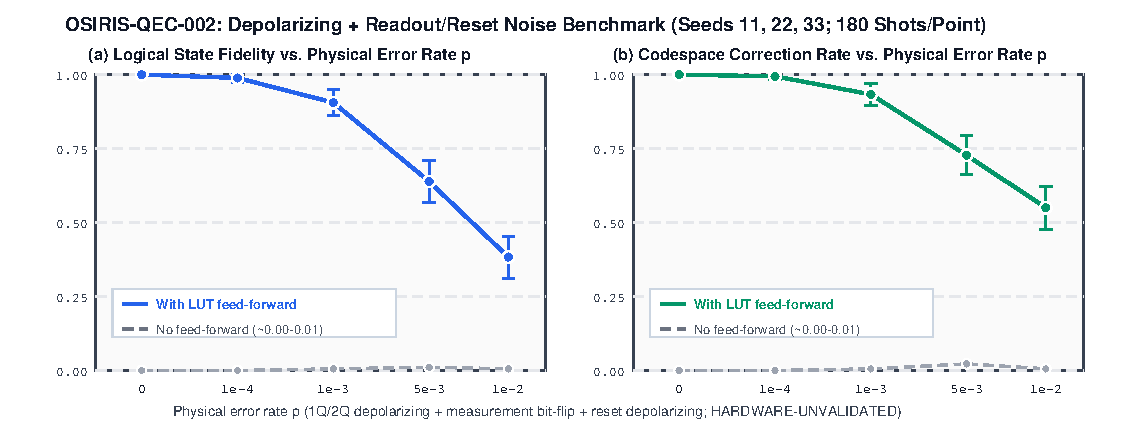
\includegraphics[width=\columnwidth]{fig2_noisy_fidelity_benchmark.pdf}
\caption{Simulated depolarizing + readout/reset noise benchmark ($180$ shots/point).}
\label{fig:bench}
\end{figure}

\begin{table}[t]
\centering
\caption{Pooled noisy preparation benchmark (simulation only).}
\label{tab:bench}
\footnotesize
\begin{tabular}{ccccc}
\toprule
$p$ & Shots & FF Fidelity & FF Codespace & No-FF Fid. \\
\midrule
0 & 180 & $1.0000 \pm 0.0000$ & $1.0000 \pm 0.0000$ & $0.0000$ \\
0.0001 & 180 & $0.9889 \pm 0.0153$ & $0.9944 \pm 0.0109$ & $0.0000$ \\
0.001 & 180 & $0.9056 \pm 0.0427$ & $0.9333 \pm 0.0364$ & $0.0056$ \\
0.005 & 180 & $0.6389 \pm 0.0702$ & $0.7278 \pm 0.0650$ & $0.0111$ \\
0.01 & 180 & $0.3833 \pm 0.0710$ & $0.5500 \pm 0.0727$ & $0.0056$ \\
\bottomrule
\end{tabular}
\end{table}

\section{16/16 Post-Prep Fault Taxonomy \& Hash-Locked H2 Gate}
Complete $16/16$ post-preparation $Y$-fault injection across $q[0..15]$ confirms $16/16$ partial $X$-syndrome detection with $0/16$ logical preservation ($F_L=0.0$; Fig.~\ref{fig:gate}). Compilation and execution enforce a preregistered artifact lock via \texttt{osiris qec}, pinning \texttt{rfc8785==0.1.4} write-ahead ledgering, \texttt{optimisation\_level=0}, post-compile ISA hash verification, \texttt{Retry-After} + jittered backoff, and a $95\%$ Wilson lower bound $>0.99$ ($512/512$, $997/1000$, $1989/2000$, $4964/5000$, $9920/10000$).

\begin{figure}[t]
\centering
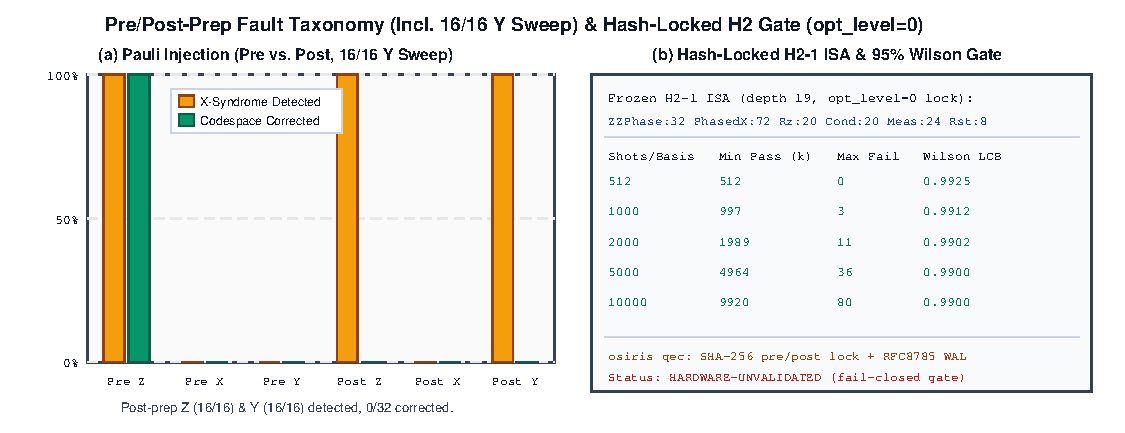
\includegraphics[width=\columnwidth]{fig3_error_taxonomy_and_wilson_gate.pdf}
\caption{$16/16$ pre/post-prep Pauli taxonomy ($0/16$ post-prep preserved) and hash-locked Quantinuum H2 Wilson ($>0.99$) gate.}
\label{fig:gate}
\end{figure}

\begin{thebibliography}{9}
\bibitem{Iqbal2024} M. Iqbal \emph{et al.}, Commun.\ Phys.\ \textbf{7}, 205 (2024); arXiv:2302.01917.
\bibitem{Wen2003} X.-G. Wen, Phys.\ Rev.\ Lett.\ \textbf{90}, 016803 (2003); A. Yu. Kitaev, Ann.\ Phys.\ \textbf{303}, 2--30 (2003).
\bibitem{Sivarajah2020} S. Sivarajah \emph{et al.}, Quantum Sci.\ Technol.\ \textbf{6}, 014003 (2020).
\bibitem{RFC8785} A. Rundgren, B. Jordan, and S. Erdtman, IETF RFC 8785 (2020).
\bibitem{Wilson1927} E. B. Wilson, J.\ Am.\ Stat.\ Assoc.\ \textbf{22}, 209--212 (1927).
\bibitem{DavisPrior} D. P. Davis, \texttt{osiris-qec} v1.0.0 (\texttt{10.5281/zenodo.24406733}) \& v1.1.0 (\texttt{10.5281/zenodo.24421051}); Companion study \texttt{OSIRIS-QEC-001}, Zenodo \texttt{10.5281/zenodo.24293756} (2026).
\end{thebibliography}
\end{document}
